\documentclass[11pt]{beamer}
\usetheme{Berlin}
\usepackage[utf8]{inputenc}
\usepackage{amsmath}
\usepackage{amsfonts}
\usepackage{amssymb}
\usepackage{graphicx}
\usepackage{multicol}
\usepackage{algorithm2e}
\useoutertheme{infolines}
\usepackage[utf8]{inputenc}
\usepackage{algpseudocode}
%\DeclareUnicodeCharacter{00A0}{ }
\usepackage{amsthm}
%\newtheorem{theorem}{Theorem}[section]
\theoremstyle{definition}
\newtheorem{defn}{}%{Definition}
\newtheorem{cor}{Corollary}[theorem]


\author{Rathijeet Bhave}
\title{Comparison Between Matching Algorithms}
%\setbeamercovered{transparent} 
%\setbeamertemplate{navigation symbols}{} 
%\logo{} 
%\institute{} 
%\date{} 
%\subject{} 
\begin{document}

\begin{frame}
\titlepage
\end{frame}

%\begin{frame}
%\tableofcontents
%\end{frame}

\begin{frame}{Outline}
This project is mainly divided into two parts.\\
\begin{itemize}


\item In \textbf{part-1} we try to find and study different algorithms that provide matching between two sets of a bipartite graph.
\item Implement them in a programming language (python in this case) to be used as a solution to various applications.
\item In \textbf{part-2} we try to compare between the results of these algorithms when same input is given to all of them.
\item Specifically to compare the extent of sub-optimality caused due to constraints like stability in matching or maximization/minimization of weights of edges
\end{itemize}
\end{frame}

\begin{frame}{Objective}
Objective of this project is to address allocation problems like 
\begin{itemize}
\item admissions of student to colleges.
\item allocation of TA's to courses.
\item allocation of committee's to students who have applied for PHD for conducting their interviews.
\end{itemize} 
\end{frame}

\begin{frame}{Students to Colleges Allocation}
\begin{itemize}
\item In this allocation we want to consider the preferences of both students and colleges.
\item In this case there should be no student-college pairing such that the student prefers some other college to which he is currently matched and the college is also better off with other student in place of him.
\item In other words we want a \textbf{stable matching.}
\end{itemize}
\end{frame}

\begin{frame}{TA to Course Allocation }
\begin{itemize}


\item In this allocation students give preferences of courses and instructors give preferences of students.
\item Even if there is a conflict of preferences, the student can be allocated to professor's choice of course.
\item In this matching the criteria is that no student should be left without a TA duty.
\item In other words we want a \textbf{maximal matching}.
\end{itemize}
\end{frame}

\begin{frame}{Invigilation Duty Allocation}
\begin{itemize}
\item The instructors give preference of centers according to their choices but exam centers does not give their choices of instructors.
\item The only constraint is a fixed number of instructors are to be allocated per exam center.           
\item The preference order of instructors can be considered as weights of edges from instructors to centers.
\item In this problem we want that no exam center should be left without enough invigilators but we also want to consider preference of invigilators as much as possible.
\item In other words we want matching to be \textbf{maximal along with the criteria that edge weights should be maximized.}
\end{itemize}
\end{frame}



\begin{frame}{Prelimenaries}

\begin{defn}{\textbf{Weighted bipartite graphs :}}
These are graphs in which each edge $(i, j)$ has a weight, or value, $w(i, j)$. The weight of matching M is the sum of the weights of edges in \textbf{M}, w(M ) = $_{e \in M}$ w(e).
\end{defn}
\begin{defn}{\textbf{Matching :}}
A matching is a subset $M \subseteq E $ such that $\forall v \in V$ at most one edge in M is incident upon v.
\end{defn}

\end{frame}

\begin{frame}{Prelimenaries}



\begin{defn}{\textbf{Maximum Matching :}}
A Maximum Matching is a matching M such that every other matching M' satisfies $|M'|\leq|M|$
\end{defn}
\begin{defn}{\textbf{Perfect Matching :}}
A perfect matching is a matching in which every vertex is adjacent to some edge in M.
Let M be a matching of G.\\*
Vertex v is matched if it is endpoint of edge in M ; otherwise v is free.
\end{defn}


\end{frame}

\begin{frame}{Prelimenaries}



\begin{defn}{\textbf{Augmenting Path :}}
An alternating path is augmenting if both end-points are free.
Augmenting path has one less edge in M than in
$E - M$ ,thus replacing the M edges by the $E - M$ ones increments size of the matching by one.
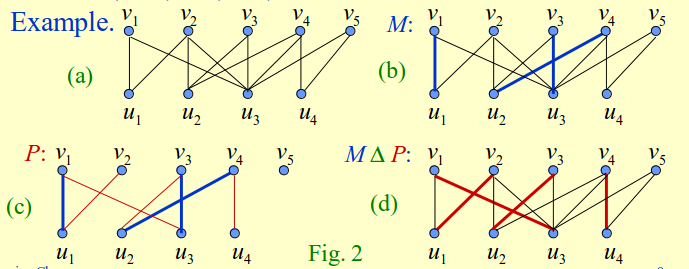
\includegraphics[width=1\textwidth]{augpath}\cite{hopcroft}
\end{defn}
\end{frame}

\begin{frame}
\begin{center}


\Huge{Hungarian algorithm}
\end{center}
\end{frame}
\section{Hungarian algorithm}
\begin{frame}{Introduction}
\begin{itemize}

\item The Hungarian method is a combinatorial optimization algorithm that solves the assignment problem in polynomial time.
\item The running time complexity of this algorithm is $\mathcal{O}(n^3)$.
\item This algorithm gives us a matching in which the edge weights are maximized/minimized as per our requirement. 
\item A matching is said to be maximum if sum of weights of all the edges in the matching is more than any other perfect matching.
\end{itemize}
\end{frame}







\begin{frame}{The Hungarian method}
\begin{enumerate}
\item Generate initial labellings $\ell$ and matching $M$ in $E_\ell$ .
\item If M is perfect, stop.\\
Otherwise pick free vertex $u \in X$.
Set $S = {u}, T = \phi$.
\item If $N_\ell (S) = T$, update labels (forcing $N_\ell (S) \neq T $).
Set $$\alpha_\ell =min_{x\in X,y \notin T} \{\ell(x) + \ell(y) - w(x, y)\}$$ and
\begin{equation*}
\ell'(v)=
\left\{ \begin{array}{ll}
\ell(v)-\alpha_\ell  \qquad \quad   & \mbox{ if } v\in s\\
\ell(v)+\alpha_\ell    &  \mbox{ if }v\in T\\
\ell(v)              &  \mbox{ otherwise }
\end{array}\right.
\end{equation*}
\item If $N_\ell (S) \neq T$ , pick $y \in \{N_\ell (S) - T\} $.
\begin{itemize}
\item If y free, (u - y) is augmenting path.
Augment M and go to 2.
\item If y matched, say to z, extend $S = S \cup \{z\}, T = T \cup \{y\}.$
\item Go to 3.
\end{itemize}
\end{enumerate}

\end{frame}

\begin{frame}
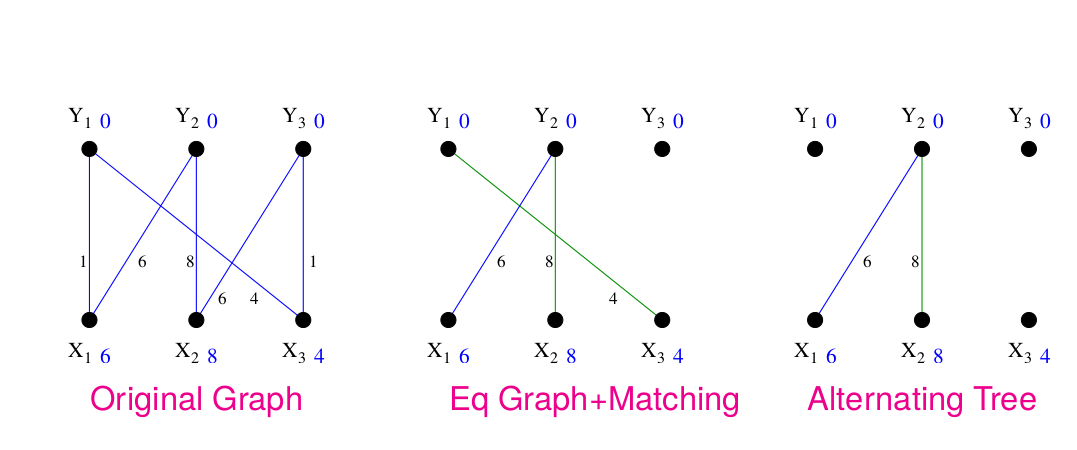
\includegraphics[scale=0.3]{hstep1}\cite{hungarian}
\begin{multicols}{2}
%\column{2in}
\begin{itemize}
\item Initial Graph, trivial labelling and associated Equality Graph.
\item Initial matching: $(x_3,y_1 ),(x_2,y_2)$
\item $S = \{x_1 \}, T = \phi $.
%\column{2in}
\columnbreak
\item Since $N_\ell (S) \neq T
\mbox{ Choose }$\\$ y_2 \in N_\ell (S)-T$.
\item $y_2$ is matched so 
$S = \{x_1 , x_2 \}, T = \{y_2 \}$.
\item At this point $N_\ell$ (S) = T , so goto 3.
\end{itemize}
\end{multicols}
\end{frame}

\begin{frame}
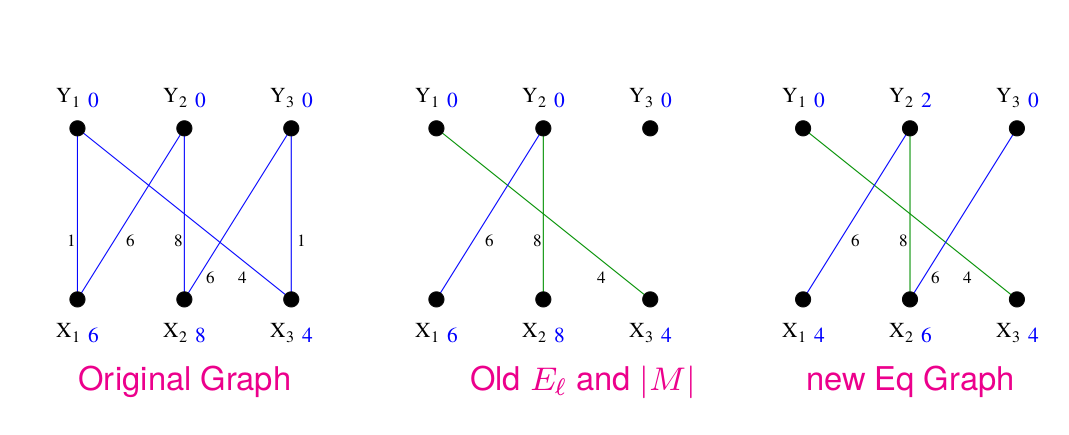
\includegraphics[scale=0.3]{hstep2}\cite{hungarian}
\begin{multicols}{2}
\begin{itemize}
\item $S = \{x_1,x_2\},T =\{y_2\}
\mbox{ and } N_\ell(S)=T $


\item calculate $\alpha_\ell$ as
\begin{scriptsize}
\begin{equation*}
\ell'(v)=\underset{x \in S,y\notin T}{min}
\left\{ \begin{array}{ll}
6+0-1,  & (x_1,y_1)\\
6+0-0,  &  (x_1,y_3)\\
8+0-0,  &  (x_2,y_1)\\
8+0-6,  &  (x_2,y_3)
\end{array}\right.
=2
\end{equation*}
\end{scriptsize}
\item Reduce labels of S by 2;
Increase labels of T by 2.
\item $ N_\ell (S) = \{y_2 , y_3 \} = \{y_2 \} = T $.
\end{itemize}
\end{multicols}
\end{frame}

\begin{frame}
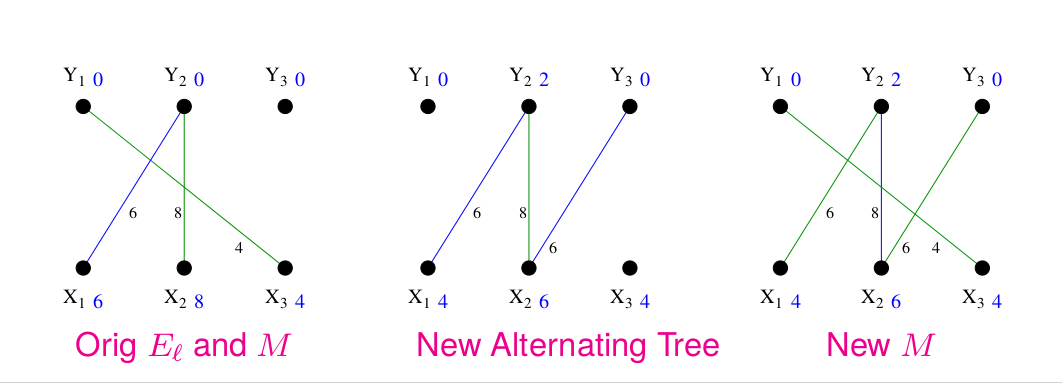
\includegraphics[scale=0.3]{hstep3}\cite{hungarian}
\begin{multicols}{2}
\begin{itemize}
\item $S = \{x_1 , x_2 \}, N_\ell (S) = \{y_2 , y_3 \}, T = \{y_2 \}$
\item Choose $y_3 \in N_\ell (S) - T$ and add it to T
\end{itemize}
\end{multicols}
\begin{itemize}
\item $y_3$ is not matched in M so
$x_1 , y_2 , x_2 , y_3$ is an alternating path.
\item After augmenting we get a mew matching \emph{M}.
\end{itemize}
\end{frame}


\begin{frame}{Complexity analysis}
In each phase of algorithm, $|M |$ increases by 1 so there are at most $\mathcal{O}(|V|)$ phases. Now we find how much work needs to be done in each phase.\\
In implementation, $\forall y \notin T$, keep track of $slack_y = \underset{x\in S}{min} \{\ell(x) + \ell(y) - w(x, y)\}.$\\
\begin{itemize}
\item Initializing all slacks at beginning of phase takes $\mathcal{O}(|V|)$ time.
\item In step 4 we must update all slacks when a vertex moves in set S. This takes  $\mathcal{O}(|V|)$ time. As at-most $|V|$ vertices can move to set S the running time of this phase will be $\mathcal{O}(|V|^2)$.
\end{itemize}
\end{frame}

\begin{frame}
\begin{itemize}

\item In step 3, $\alpha_\ell = \underset{y\in T}{min}\mbox{ } slack_y$ and can therefore be calculated in $\mathcal{O}(|V|)$ time from the slacks. This in worst case would be done at most $|V |$ times per phase.This is because only $|V|$ vertices can be moved to set S. So this step also takes $\mathcal{O}(|V|^2)$ time.
\item There are $|V |$ phases and $\mathcal{O}(|V |^2 )$ work per phase. so the total running time is $\mathcal{O}(|V |^3 )$
\end{itemize}
\end{frame}

\begin{frame}
$\Large{Input Matrix}=
\begin{pmatrix}
7 & 2 & 8\\
8 & 0 & 2\\
4 & 8 & 7
\end{pmatrix}$
\end{frame}

\begin{frame}
\begin{center}
\huge{Hopcroft Karp Algorithm}
\end{center}
\end{frame}

\section{Hopcroft Karp Algorithm}
\begin{algorithm}[H]%\frametitle{Pseudo Code}
\begin{itemize}


\item In this algorithm we find a maximal family of vertex-disjoint shortest-length augmenting paths and augment all of them together in a single stage.
\item This improvement will help us to
bring the time complexity down to $\mathcal{O}(n ^{2.5} )$.
\end{itemize}
The algorithm is as follows.
%\begin{algorithm}
\caption{Hopcroft Karp Algorithm}
M = $\phi$\\
\While {there is an M -augmenting path}{ 
	Find a maximal family $F$ of vertex-disjoint 		shortest M -augmenting paths;\\
	set $M = M \oplus F$ }
\Return M

\end{algorithm}



\begin{frame}
\begin{theorem}\label{name}
M is a maximum matching if and only if there is no augmenting path relative to M.
\end{theorem}


\begin{theorem}\label{upprbndlenpath}
Let M be a matching. Suppose $|M|= r$, and suppose that the cardinality of a maximum matching is s, $s > r$. Let n be the total number of vertices. Then there exists an augmenting path
relative to M of length $\leq \frac{n}{s-r}-1$.
\end{theorem} 
\textbf{Hint}  $$(s-r)(\ell +1) \leq n.$$
\end{frame}

\begin{frame}
\begin{theorem}\label{minlenshpath}
Let M be a matching, P a shortest augmenting path relative to
M, and $P'$ an augmenting path relative to $M \oplus P$. Then
$$|P'| \geq |P| + 2|P \cap P'|$$.\\
\end{theorem} 
\textbf{Hint}  $$|M \oplus N|=|P\oplus P'|=|P|+|P'|-2|P \cap P'| \geq |P1|+|P2| \geq 2|P|$$.


\begin{cor} Let P be a shortest augmenting path relative to a matching M, and Q be a shortest augmenting path relative to $M \oplus P$. Then, if $|P| = |Q|$, the paths P and Q must be node-disjoint.
\end{cor}




\end{frame}

\begin{frame}{Finding augmenting paths}\label{construct_graph}
\begin{cor} After each phase the shortest augmenting path is strictly longer than the shortest augmenting path of the previous phase.
\end{cor}

\begin{theorem}A maximal set of vertex disjoint minimum length augmenting paths can be found in $\mathcal{O}(m)$ time.	
\end{theorem}

\end{frame}



\begin{frame}{Python Implementation}
\textbf{First step:} To find the length of minimum length augmenting path.\\
Construct a graph $G_i$ in the same way as `H' was constructed in \ref{construct_graph}.\\
From $G_i$, construct a subgraph $G_{i'}$ described below.\\
Let $L_0$ be the set of free nodes relative to $M_i$ in A and define $L_j (j > 0)$ as follows:
$$E_{j-1} = \{u \rightarrow v \in E(G_i)\mbox{ } | \mbox{ } u \in  L_{j-1}, v \in L_0 \cup L_1 \cup ...\cup L_{j-1}\}$$
$$L_j = {v \in V(G_i) |\mbox{ for some u}, u \rightarrow v \in E_{j-1}}.$$
\end{frame}

\begin{frame}


Define $j* = min\{j | L_j \cap \{\mbox{free nodes in B}\} \neq \phi\}$\\
$G_i'$ is formed with $V(G_i')$ and $E(G_i')$ as defined below.\\
If $j* = 1$, then 
	$$V(G_i') = L_0 \cup (L_1 \cap \mbox{\{free nodes in B\}})$$
	$$E(G_i') = \{u \rightarrow v | u \in L_0 \mbox{ and } v \in \{\mbox{free nodes in B}\}\}.$$
If $j* > 1$, then
	$$V(G_i') = L_0 \cup L_1 \cup ... \cup L_{j*-1} \cup (L_{j*} \cap \{\mbox{free nodes in 	B}\}),$$
	$$E(G_i') = E_0 \cup E_1 \cup ... \cup E_{j*-2} \cup \{u \rightarrow v | u \in L_{j*-1} and 	v \in \{\mbox{free nodes in B}\}.$$


\end{frame}

\begin{frame}
\textbf{Second step:} To find maximal set of shortest augmenting paths.\\
Data structure stack is used to temporarily store the augmenting paths. c-list of a vertex `v' is defined as all the vertices which are connected to `v' through an edge. The algorithm is as follows.
\end{frame}

\begin{algorithm}[H]
\begin{scriptsize}

\caption{Augmrnting path algorithm}
let v be the first element in $L_0$;
push(v, stack); mark v;\\
\While {stack is not empty}{
	v $:=$ top(stack);\\
	\While {c-list(v) $\neq \phi$}{
		let u be the first element in c-list(v);\\
		\eIf {u is marked}{
			remove u from c-list(v)}
		{
			push(u, stack); \\
			mark u; 
			v := u;\\
		}
	}
	\eIf {v is neither in $L_{j^*}$ nor in $L_0$}		{ 			pop(stack)}
	{
		\If {v is in $L_{j^*}$}{
			output all the elements in stack;
				(all the elements in stack 						make up an augmenting path.)\\
			remove all elements in stack;\\
			let v be the next element in $L_0$;\\
			push(v, stack);
			mark v;
			}
	}
}
\end{scriptsize}
\end{algorithm}

\begin{frame}
%\includegraphics[width=10cm,height=10cm,keepaspectratio]{image}
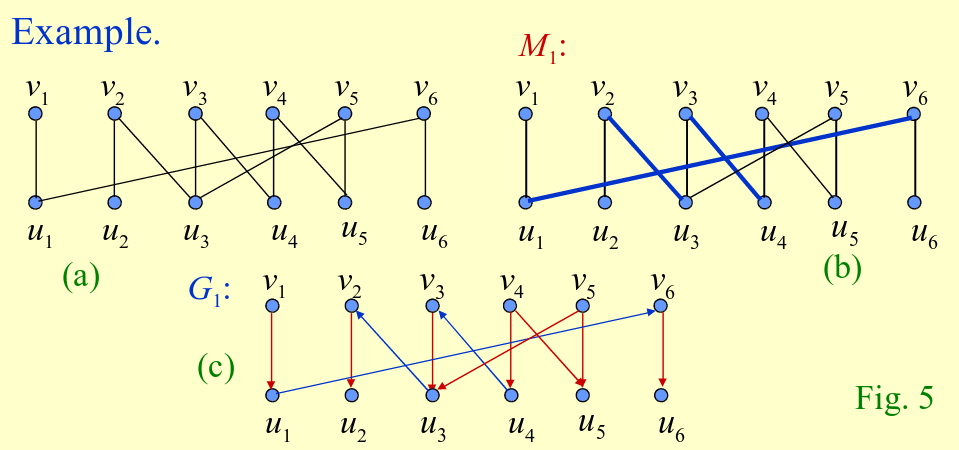
\includegraphics[width=12cm,height=4cm]{hopstep1}\cite{hopcroft}\\
\begin{itemize}
\item $L_0 = \{v_1, v_4, v_5\}$
\item $E_0 = \{(v_1, u_1), (v_4, u_4), (v_4, u_5), (v_5, u_3), (v_5, u_5)\}$
\item $L_1 = \{u_1, u_3, u_4, u_5\},\mbox{ }j^*=1$.
\item $V(G_1’) = \{v_1, v_4, v_5\}\cup\{u_5\}$
\item	$E(G_1’) = \{(v_4, u_5), (v_5, u_5)\}$
\end{itemize}
\end{frame}

\begin{frame}
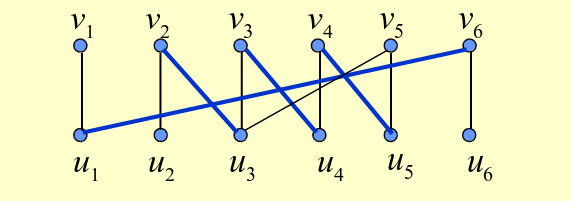
\includegraphics[width=12cm,height=4cm]{hopstep2}\cite{hopcroft}\\
\begin{itemize}
\item $v_4 \rightarrow u_5 \mbox{ and } v_5 \rightarrow u_5 \mbox{ are augmenting paths out of which }v_4 \rightarrow u_5 \mbox{ is selected }$
\item $M_2 = M_1 \oplus \{v_4 \rightarrow u_5\}$
\end{itemize}
\end{frame}

\begin{frame}
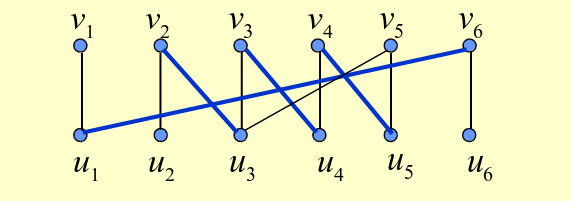
\includegraphics[width=12cm,height=4cm]{hopstep2}\cite{hopcroft}\\
\begin{multicols}{2}
\begin{itemize}
\item $L_0=\{v_1,v_5\}$
\item $E_0=\{v_1,u_1),(v_5,u_3),(v_5,u_5)\}$
\item $L_1=\{u_1,u_3,u_5\}$
\item $E_1=\{(u_1,v_6),(u_3,v_2),(u_5,v_4)\}$
\item $L_2=\{v_2,v_4,v_6\}$
\item $E_2=\{(v_2,u_2),(v_4,u_4),(v_6,u_6)\}$
\item $L_3=\{u_2,u_4,u_6\}$

\end{itemize}
\end{multicols}
\end{frame}

\begin{frame}
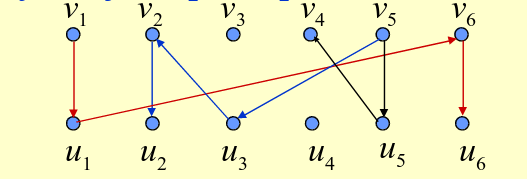
\includegraphics[width=12cm,height=4cm]{hopstep3}\cite{hopcroft}\\
\begin{itemize}
\item $j^*=3$
\item $V(G_2')=L_0 \cup L_1 \cup L_2 \cup \{u_2,u_6\}$
\item $E(G_2')=E_0 \cup E_1 \cup \{(v_2,u_2),(v_6,u_6)\}$
\item Start a DFS from $v_1,v_5$ to obtain augmenting paths.
\item Final matching = $\{(v_1,u_1),(v_6,u_6),(v_2,u_2),(v_5,u_3),(v_3,u_4),(v_4,u_5)\}$
\end{itemize}
\end{frame}


\begin{frame}{Complexity analysis}
\begin{itemize}


\item Algorithm of finding a maximal set of vertex disjoint shortest length augmenting paths can be implemented in $\mathcal{O}(m)$ time.
\item Let M be the matching obtained after exactly $\sqrt{n}$ phases.
\item Each augmenting path from now on is atleast of length $2\sqrt{n}+1$. This is because after each phase the length of shortest augmenting path increases by atleast 2.
\item Let $M^*$ be the maximum matching. So there exists atleast $|M^*|-|M|$ vertex disjoint augmenting paths. 
\item The length of shortest augmenting path will utmost be $\frac{n}{|M^*|-|M|} -1$.
\end{itemize}
\end{frame}

\begin{frame}
\begin{itemize}

\item Following inequality holds $$\sqrt{n} \leq (\mbox{length of shortest M -augmenting path})\leq\frac{n}{|M^*|-|M|}$$
and so on simplification we get $$|M^*| - |M | \leq \sqrt{n}$$
From this point onwards, we need at most $\sqrt{n}$ more iterations,
\item Thus overall no more than $2\sqrt{n}$ iterations are needed.
\item The overall running time can now be written as $\mathcal{O}(\sqrt{n}m)$.
\item In a bipartite graph the number of edges cannot be more than $n^2/4$. So the overall running time would be $$\mathcal{O}(\sqrt{n}\times n^2) = \mathcal{O}(n^{2.5})$$
\end{itemize}
\end{frame}

\begin{frame}
\begin{center}
\huge{Gale Shapely Algorithm}
\end{center}
\end{frame}
\section{Gale Shapely Algorithm}
\begin{frame}{Introduction}
This algorithm gives solution to Stable matching problem.
A matching is stable whenever it is not the case that both the statements hold true:
\begin{enumerate}
\item some given element A of the first matched set prefers some given element B of the second matched set over the element to which A is already matched.
\item B also prefers A over the element to which B is already matched.
Algorithm for finding solution of stable marriage problem is given below.
\end{enumerate}

\end{frame}

\begin{algorithm}[H]

\caption{Gale Shapely algorithm}
Initialize all $m \in M$ and $w \in W$ to free\\
\While {$\exists$ free man m who still has a woman w to propose to }{
	w = m's highest ranked woman to whom he has not yet proposed\\
	\eIf {w is free}
	{
		(m, w) become engaged
	}
    {
    		$*$(some pair (m', w) already exists)$*$\\
		\eIf {w prefers m to m'}
		{
			(m, w) become engaged\\
			m' becomes free
		}
		{
			(m', w) remain engaged
    		}
    	}
}
\end{algorithm}



\begin{frame}
$\Large{malepref=}
\begin{pmatrix}
2&4&1&3\\
3&1&4&2\\
2&3&1&4\\
4&1&3&2\\
\end{pmatrix}
\Large{femalepref=}
\begin{pmatrix}
2&1&4&3\\
4&3&1&2\\
1&4&3&2\\
2&1&4&3\\
\end{pmatrix}$\\ 
First round : $1\rightarrow free,2\rightarrow 3,3\rightarrow 2,4\rightarrow 4$\\
Second round: $1\rightarrow 4,2\rightarrow 3,3\rightarrow 2,4\rightarrow free$\\
Third round: $1\rightarrow 1,2\rightarrow 3,3\rightarrow 2,4\rightarrow 1$\\
\begin{center}
$
\Large{answer=}
\begin{pmatrix}
1&1\\
2&4\\
3&2\\
4&3
\end{pmatrix}$
\end{center}
\end{frame}

\begin{frame}{Complexity Analysis}
\begin{itemize}


\item The worst case for this algorithm would be when one man gets his last preference and all others get their penultimate preferences i.e when the number of proposals are maximum.
\item Assume there are 'n' men and 'n' women. Each iteration has atleast one proposal.
\item Only an engaged women can reject. So no man can be rejected by all women.
\item No man proposes twice to same women.So total number of proposals are upper bounded by $n^2$.
Hence the running time of this algorithm is $\mathcal{O}(n^2)$.
\end{itemize}
\end{frame}

\begin{thebibliography}{9}

\bibitem{hopcroft}
John E.Hopcroft
and 
Richard M.Karp
  \emph{AN $n^{5/2}$ Algorithm For Maximum Matchings
In Bipartite Graphs}

\bibitem{hungarian}
H.
W.
Kuhn
\emph{The Hungarian Method For The
Assignment Problem}
Bryn Yaw College 1955

\bibitem{gale}
Dan Gusfield and Robert W.Irving,
\emph{Stable Marriage Problem Structure and}
Oxford Handbook of Innovation
The MIT Press
Cambridge Massachusetts London England
1989,




\end{thebibliography}
\begin{frame}
\begin{center}



\Huge{THANK YOU}
\end{center}
\end{frame}
\end{document}
